\documentclass[runningheads]{llncs}
%
\usepackage[T1]{fontenc}
\usepackage{graphicx}
\usepackage{amsmath, amssymb}
\usepackage{esvect} % For enhanced vector notation
\usepackage{bm} % For bold vectors if needed
\usepackage{booktabs}
\usepackage{hyperref}
\usepackage{color}
\usepackage{float}
\usepackage{placeins}
\usepackage{needspace}  % Keeps the preceding paragraph with the figure
\usepackage{tikz}
\usetikzlibrary{arrows.meta,positioning}

\definecolor{RetrievalNavy}{RGB}{24,49,74}
\definecolor{RetrievalTeal}{RGB}{0,122,128}
% Custom configuration for hyperref
\hypersetup{
    colorlinks=true,
    linkcolor=blue,
    citecolor=blue,
    urlcolor=blue
}

\begin{document}
\raggedbottom % avoid stretched vertical whitespace on pages with large floats
%
\title{LLM Agents for Interlinked and Personalised Knowledge Bases}
%
\titlerunning{LLM Agents for Personalised Knowledge Bases}
%
\author{Muhammed Furkan Kaya}
%
\authorrunning{M. F. Kaya}
%
\institute{Vrije Universiteit Amsterdam\\
\email{m.f.kaya@student.vu.nl}\\
\textbf{Supervisor:} Emile van Krieken\\
\textbf{Second Assessor:} Frank van Harmelen
}
%
\maketitle              % typeset the header of the contribution
%
\begin{abstract}

Personal Knowledge Management systems can help researchers organise
scientific literature as interconnected notes, but manually extracting
metadata, summarising papers, and maintaining links between related
documents remains time-consuming. This thesis develops and evaluates a
modular pipeline of specialised LLM-based components that transforms
academic PDFs into structured, interlinked Obsidian Markdown notes.

The pipeline was evaluated on a focused personal research collection of
40 academic papers. Retrieval was compared across three configurations:
Flat RAG over PDF-derived text chunks, Structured RAG over generated
Markdown notes, and Link-Expanded RAG, which applies a one-hop
semantic-link score boost. The evaluation also measured bibliographic
metadata extraction, topic-label alignment with expert-authored
annotations, explicit citation-reference extraction, and the qualitative
usefulness of generated notes.

Structured RAG did not consistently outperform the chunk-based baseline,
although it achieved the highest observed MRR@5. Link-Expanded RAG achieved the highest observed Recall@5, but the
difference in retrieval coverage was small and was not tested for
statistical significance. Title extraction reached a 97.5\% exact-match rate,
while strict agreement with expert-authored topic labels remained low. A
separate canonicalised topic evaluation produced higher alignment, but
the two protocols are not directly comparable. Citation-reference extraction achieved a precision of 0.84, recall of
0.74, and an F1-score of 0.79. In
an exploratory expert evaluation of five notes, the overall mean rating
was 3.35 out of 5, with factual faithfulness rated highest and
core-contribution coverage rated lowest.

Overall, the pipeline automated several knowledge-base construction
tasks with mixed levels of success. The pipeline achieved its strongest results on title matching, author
extraction, and citation-reference extraction, but structured
LLM-generated notes did not automatically improve retrieval; topic
alignment, incomplete citation coverage, and expert-level note coverage
remain important limitations.

\keywords{Retrieval-Augmented Generation \and Personal Knowledge Graphs
\and Obsidian \and LLM Agents \and Information Retrieval}
\end{abstract}
%
%
%
\section{Introduction}
\label{sec:intro}

\subsection{Context and Motivation}

Academic research increasingly depends on the ability to organise,
retrieve, and connect information across large collections of papers.
Researchers must not only store documents, but also track methods,
datasets, assumptions, findings, and relationships between related work.
As collections grow, this process can become difficult to maintain
manually.

Personal Knowledge Management (PKM) systems such as Obsidian, Logseq,
and Roam Research support this process by representing knowledge as
interconnected notes rather than as isolated documents. Balog and Kenter
define a Personal Knowledge Graph (PKG) as a resource containing
structured information about entities that are personally related to its
user~\cite{balog2019personal}. In this thesis, this concept is
operationalised as a graph in which structured Markdown paper notes
represent nodes and explicit Markdown wiki-links
(\texttt{[[Note Target]]}) represent directed relationships between
notes.

A well-maintained academic PKG can serve as an externalised research
memory that reflects a researcher's own interests, terminology, and
organisational preferences. However, constructing such a graph requires
repeated manual work: obtaining papers, reading them, extracting
bibliographic metadata, summarising contributions, and identifying
relationships with previously stored literature. When this process is
not maintained consistently, personal research collections can devolve
into folders of weakly connected PDFs and notes, limiting the practical
value of graph-based organisation.

\subsection{Problem Statement}

Large Language Models (LLMs) offer a possible way to automate parts of
academic knowledge-base construction by extracting bibliographic
metadata, generating structured summaries, and proposing links between
related papers. However, it remains unclear whether transforming raw
academic PDFs into interlinked, agent-generated notes consistently
improves downstream Information Retrieval (IR) compared with flat
chunk-based retrieval, or whether its benefits are more apparent in the
structured notes and extracted information produced by the pipeline.

Retrieval-Augmented Generation (RAG) combines a generative language model
with information retrieved from an external document
collection~\cite{lewis2020retrieval}. In the Flat RAG baseline
implemented in this thesis, PDF-derived plain text is divided into
sequential 512-token chunks with a 50-token overlap. Each chunk is
embedded independently. For each query, a paper is assigned the
similarity score of its highest-scoring chunk, after which the
highest-ranked papers are returned. Although this approach is simple and
computationally practical, it introduces two limitations relevant to
personal academic knowledge bases:

\begin{enumerate}
\item \textbf{Context Fragmentation:} A coherent argument,
contribution, or methodological description may be divided across
arbitrary chunk boundaries, causing retrieved units to contain
incomplete context~\cite{sarthi2024raptor}.

\item \textbf{Loss of Inter-Document Context:} Independent vector
retrieval does not explicitly incorporate graph structure or semantic
relationships between papers during document ranking
~\cite{edge2024local,gutierrez2024hipporag}.
\end{enumerate}

To investigate these limitations, this thesis implements a modular
LLM-based ingestion pipeline that transforms academic PDFs into
structured, Obsidian-compatible Markdown notes and generates typed
semantic wiki-links between papers. Retrieval is evaluated using three
configurations: Flat RAG over PDF-derived text chunks, Structured RAG
over agent-generated notes, and Link-Expanded RAG, which applies an
additional score boost to papers connected to the initially retrieved
seed papers through the generated wiki-link graph. This design evaluates
the graph-expansion step separately from structured-note retrieval, while
the comparison between Flat RAG and Structured RAG captures the combined
effect of changing from chunk-level PDF text to paper-level generated
notes.

\subsection{Research Questions and Hypotheses}
\label{sec:rqs}

The primary objective of this thesis is to evaluate whether a modular
LLM-based pipeline can transform a flat PDF collection into a structured,
interlinked personal academic knowledge base, and whether this
transformation improves retrieval compared with a Flat RAG baseline.
Supporting research questions evaluate the accuracy of metadata
extraction, topic-label alignment, explicit citation-reference
extraction, and the qualitative usefulness of the generated notes.

\begin{quote}
\textit{To what extent can a modular pipeline of specialised LLM-based
components improve retrieval in a personal knowledge base by generating
structured notes and inter-note links, compared with a Flat RAG
baseline?}
\end{quote}

This objective is addressed through four research questions and their
corresponding hypotheses.

\subsubsection{RQ1: Retrieval Performance}

Does retrieval from structured, LLM-generated Markdown notes, with or
without graph-informed link expansion, improve search quality compared
with retrieval from flat PDF chunks?

\begin{itemize}
\item[\textbf{H1:}] Structured RAG is expected to improve retrieval over
Flat RAG by preserving paper-level context and reducing fragmentation.
Link-Expanded RAG is further expected to improve retrieval by using
semantic relationships represented through inter-note wiki-links.
\end{itemize}

\subsubsection{RQ2: Metadata and Topic Extraction Accuracy}

How accurately can the pipeline extract bibliographic metadata compared
with reference records, and how well do its generated topic labels align
with expert-authored annotations?

\begin{itemize}
\item[\textbf{H2:}] Bibliographic metadata is expected to show higher
agreement with reference records than generated topic labels show with
expert-authored annotations, because metadata fields are more explicit
and less dependent on personal vocabulary choices.
\end{itemize}

\subsubsection{RQ3: Citation Reference Extraction Accuracy}

How accurately can the citation-extraction pipeline recover explicit
bibliographic references from academic papers compared with Semantic
Scholar reference records?

\begin{itemize}
\item[\textbf{H3:}] The citation-extraction pipeline is expected to
achieve high precision, while incomplete recovery of individual
bibliography entries is expected to result in lower recall.
\end{itemize}

\subsubsection{RQ4: Qualitative Expert Evaluation of Generated Notes}

How does a domain expert assess the factual faithfulness,
core-contribution coverage, structure and readability, and rediscovery
utility of the LLM-generated notes?

\begin{itemize}
\item[\textbf{H4:}] The generated notes are expected to receive mean
ratings above the neutral midpoint of 3 out of 5 across all four
evaluation dimensions.
\end{itemize}

% ============================================================

\section{Literature Study}
\label{sec:literature}

This section reviews research on retrieval representations,
LLM-supported personal knowledge management, academic information
extraction, and human evaluation of generated summaries. These areas
inform the design and evaluation of the proposed pipeline.

\subsection{Retrieval Representations and Graph Expansion}

Retrieval-Augmented Generation (RAG) supplements a language model with
information retrieved from an external document
collection~\cite{lewis2020retrieval}. A common implementation embeds
fixed-size document chunks and ranks them by similarity to a query.
Although practical, chunking can split related arguments, methods, or
findings across retrieval units. RAPTOR addresses this by clustering and
summarising chunks into a hierarchical retrieval
tree~\cite{sarthi2024raptor}.

Graph-based RAG methods incorporate explicit relationships between
information units. GraphRAG constructs entity-relation graphs and
community summaries for query-focused
summarisation~\cite{edge2024local}, while HippoRAG applies Personalised
PageRank over a concept graph for associative and multi-hop
retrieval~\cite{gutierrez2024hipporag}. GraphRAG-Bench assesses graph
construction, knowledge retrieval, and answer generation separately,
providing evaluation across the complete GraphRAG
pipeline~\cite{xiao2025graphragbench}. These findings motivate the
comparison between flat chunks, structured notes, and lightweight
one-hop link expansion used in this thesis.

\subsection{LLM-Supported Personal Knowledge Management}

Personal Knowledge Graphs (PKGs) organise information through
personally meaningful relationships~\cite{balog2019personal}. In
academic settings, Markdown-based tools such as Obsidian can support a
lightweight PKG-like representation in which notes act as nodes and
wiki-links encode directed relationships between them. Recent practical
systems demonstrate how LLMs can automate parts of this construction
process. The open-source \textit{My-Brain-Is-Full-Crew} project uses
coordinated components to structure, search, connect, and maintain
notes within an Obsidian vault~\cite{mybrainisfullcrew}. As a software
repository rather than a peer-reviewed study, however, it does not
establish whether its outputs are accurate or whether they improve
retrieval. This gap between practical feasibility and controlled
evaluation directly motivates the present work.

\subsection{Academic Information Extraction}

Specialised systems such as CERMINE have demonstrated that scientific
documents can be converted into structured metadata using dedicated
document-analysis pipelines~\cite{tkaczyk2015cermine}. LLM-based
generative information extraction offers a more flexible alternative
by prompting a language model to produce structured fields directly
from source text~\cite{xu2024large}. Bibliographic metadata such as
titles, years, venues, and author names are typically stated
explicitly, whereas semantic topic labels require interpretation and
may vary between annotators. This distinction motivates separate
evaluation protocols for bibliographic fields and topic-label alignment
in RQ2. For RQ3, the focus shifts to explicit bibliographic references
extracted from paper reference sections, compared against records from
the Semantic Scholar Academic Graph~\cite{kinney2023semantic}. This
tests reference recovery from raw text rather than prediction of
implicit semantic relationships.

\subsection{Human Evaluation of Generated Notes}

Automatic metrics alone cannot determine whether a pipeline-generated
note is factually reliable, readable, or useful to a researcher. Human
evaluation therefore remains important in summarisation research.
SummEval demonstrates the use of expert judgements to assess multiple
quality dimensions, including consistency, relevance, coherence, and
fluency~\cite{fabbri2021summeval}. Drawing on this multidimensional
evaluation principle, RQ4 uses an exploratory qualitative expert
evaluation of five LLM-generated notes, covering factual faithfulness,
core-contribution coverage, structure and readability, and utility for
rediscovery.

\subsection{Synthesis and Research Gap}

The reviewed work shows that hierarchical and graph-based retrieval
methods can incorporate broader context or explicit relations than flat
retrieval, but add construction, summarisation, or traversal stages.
Scientific information extraction and citation-reference recovery also
require task-specific evaluation methods. For generated notes, automatic
metrics alone cannot capture factual faithfulness, coverage, readability,
or rediscovery utility, motivating expert assessment. However, the
reviewed literature provides limited evidence on evaluating these
components together in lightweight Markdown-native academic PKM
workflows. This motivates separate retrieval and extraction protocols,
alongside an exploratory expert assessment.

% ============================================================
\section{Methodology}
\label{sec:methodology}
% Placeholder for Section 3: Methodology
% Guideline: Describe the approach taken to investigate the research question, including 
% methods, models, or frameworks applied. Present research process steps and reasoning, 
% making assumptions explicit. Detail the data used (structure, preprocessing, limitations).

This section describes the academic-paper corpus, the modular
LLM-based ingestion pipeline, the three retrieval configurations, and
the evaluation procedures used to address RQ1--RQ4. The study combines
quantitative evaluations of retrieval and information-extraction
performance with an exploratory expert evaluation of the generated
notes.

\subsection{Corpus and Data Preparation}
\label{sec:corpus}

The evaluation corpus consists of 40 academic papers. Eighteen papers
were added through external arXiv-based collection for retrieval, RAG,
agentic memory, and neuro-symbolic topics. The remaining 22 papers
overlapped with the supervisor's expert-authored Obsidian vault. Part
of this vault source is publicly available through the
\texttt{academic-obsidian} repository~\cite{vankriekenAcademicObsidian},
while additional vault notes were provided privately for this project.
The collection includes both published papers and preprints covering
several areas of artificial intelligence relevant to the knowledge base.
Each paper is identified by its arXiv identifier and represented through
three aligned artefacts: the original PDF, PyMuPDF-extracted plain text
stored in JSON format, and an agent-generated Markdown note.

Before evaluation, automated preflight checks verified that the
extracted texts, generated notes, retrieval queries, and relevance
labels referred to the same set of document identifiers. The generated
notes and semantic links were frozen before the final evaluations.
Consequently, the later RQ3 citation-extraction experiment could not
modify the retrieval indexes, note contents, or semantic links evaluated
in RQ1 and RQ2.

Different research questions required different subsets because the
availability of expert annotations and external gold records varied
across the corpus. Table~\ref{tab:evaluation_subsets} summarises the
datasets used by each evaluation.

\begin{table}[htbp]
    \centering
    \caption{Corpus subsets used for the four research questions.}
    \label{tab:evaluation_subsets}
    \begin{tabular}{p{0.48\linewidth} p{0.39\linewidth}}
        \toprule
        \textbf{Evaluation} & \textbf{Dataset} \\
        \midrule

        RQ1 retrieval evaluation
        & 40 papers and 40 queries \\

        RQ2 bibliographic metadata
        & 40 papers \\

        RQ2 strict topic evaluation
        & 22 papers with expert topic annotations \\

        RQ2 canonicalised topic evaluation
        & 7 development papers and a 15-paper evaluation subset \\

        RQ3 citation-reference evaluation
        & 37 scored papers \\

        RQ4 expert evaluation
        & 5 generated notes \\

        \bottomrule
    \end{tabular}
\end{table}

The corpus is a focused research collection rather than a random sample
of the broader academic literature. The reported results therefore
characterise the behaviour of the pipeline within this collection and
should not be interpreted as population-level performance estimates
across all scientific domains.

\subsection{Multi-Agent Ingestion Pipeline}
\label{sec:agent_pipeline}

In this thesis, an \emph{agent} is a task-specialised LLM component
with a predefined input specification, prompt, and output schema, executed in a
predetermined workflow without independent planning. \emph{Multi-agent
pipeline} therefore denotes a composition of specialised components
rather than an autonomous multi-agent system.

After shared PDF text extraction, the workflow separates into two
processing paths. The main ingestion path generates structured Markdown
notes and semantic links. A separate citation-extraction path processes
explicit bibliography entries for RQ3 after the RQ1 and RQ2 artefacts
have been frozen. Its batching, parsing, and fallback procedures are
defined in Section~\ref{sec:rq3_method}.

The main ingestion path contains three sequential stages:

\begin{enumerate}
    \item \textbf{Metadata extraction.}
    The Metadata Agent extracts bibliographic attributes such as title,
    authors, publication year, venue, and paper identifiers. It also
    extracts semantic fields including topics, concepts, methods,
    datasets, and evaluation metrics. The resulting values are stored as
    structured JSON and subsequently inserted into the YAML frontmatter
    of the generated note.

    \item \textbf{Structured note generation.}
    The Structured Note Agent combines the extracted paper text and
    metadata to produce a standardised Markdown note. Each note contains
    sections describing the research problem, methodology, datasets or
    experimental setup, evaluation metrics, principal findings, and
    limitations.

    \item \textbf{Semantic link generation.}
    The Semantic Link Agent compares each generated note with candidate
    notes from the local corpus and proposes typed, directional
    wiki-links. The supported relationship types include shared topics
    and methods, extensions, comparisons, contradictions, datasets, and
    evaluation relationships. For each target note, the candidate set consisted of all other
    generated notes in the 40-paper corpus, giving 39 candidates; no
    embedding-based preselection was used at this stage. The agent
    receives the target note's title, frontmatter, and summary together
    with metadata and summaries for the candidate notes. The prompt requests typed JSON link proposals with model-reported confidence scores. The implementation retains proposals with scores of
    at least \(0.6\), using this value as a fixed operational filter rather
    than a calibrated probability. Accepted links are appended under the
    dedicated \texttt{\#\# Generated Links} heading and later consumed by
    Link-Expanded RAG.
\end{enumerate}

The Citation Link Agent extracts explicit bibliography records rather
than conceptual relationships. Records may contain a title, authors,
year, venue, DOI, arXiv identifier, or Semantic Scholar identifier.
External references remain valid outputs, while matches within the
40-paper corpus can additionally receive Obsidian wiki-links.

Figure~\ref{fig:pipeline_architecture} summarises the complete ingestion
architecture and distinguishes semantic relationship generation from
explicit bibliography extraction.

\begin{figure}[H]
    \centering
    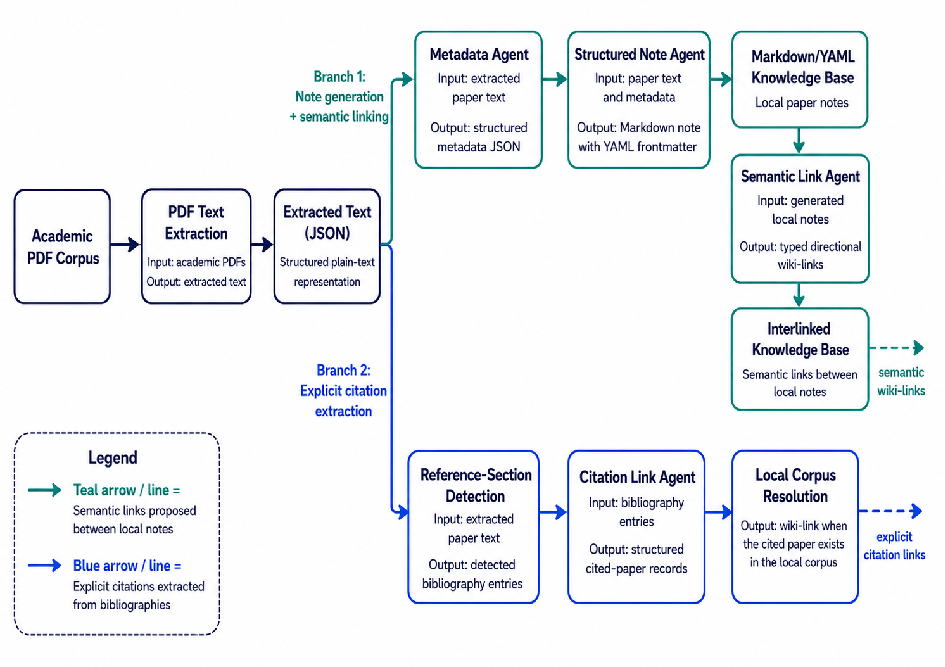
\includegraphics[
        width=\linewidth,
        height=0.62\textheight,
        keepaspectratio
    ]{figures/pipeline_architecture.pdf}
    \caption{Architecture of the modular academic-paper ingestion pipeline.
The main path generates structured notes and semantic links. The
separate citation-extraction path extracts explicit bibliography
records; references matching papers in the local corpus can additionally
be resolved to wiki-links.}
    \label{fig:pipeline_architecture}
\end{figure}

\noindent\textbf{LLM configuration and prompt control.}
All LLM-backed pipeline stages used a shared Gemini Flash-family API
wrapper with temperature fixed at \(0.0\). The metadata-extraction,
note-generation, and semantic-link instructions were stored as separate
version-controlled prompt templates defining the required JSON or
Markdown output schemas. Citation extraction likewise used a
version-controlled prompt defining the required reference-record
structure.

The Metadata Agent received the first 8,000 characters of extracted
paper text, while the Structured Note Agent received up to 12,000
characters. The Semantic Link Agent received the target note's
frontmatter, the first 2,000 characters of its summary, and up to
500 characters from each candidate summary. The final RQ3 pipeline was
an exception to these ingestion-stage input limits: it attempted to
process the complete detected bibliography section after dividing it
into batches of at most 30 entries.

Detailed model-pool provenance, caching procedures, artefact retention,
and the endpoint-logging limitation are reported in
Section~\ref{sec:reproducibility}.

\subsection{Retrieval Representations and Embedding Model}
\label{sec:retrieval_representations}

Flat RAG uses PDF-derived plain text, whereas Structured RAG and
Link-Expanded RAG use generated Markdown notes. RQ1 evaluates retrieval
only; no downstream answer-generation model is applied.

All configurations use the SentenceTransformers library
~\cite{reimers2019sentence} to load the
\path{nomic-ai/nomic-embed-text-v1.5} model
~\cite{nussbaum2024nomic}, with \texttt{search\_query:} and
\texttt{search\_\allowbreak{}document:} prefixes. Queries and document
units are independently encoded by the same pretrained model in a
bi-encoder setup and compared using cosine similarity
~\cite{reimers2019sentence,karpukhin2020dense}. No embedding model is
trained or fine-tuned.

Let \(E(x)\) denote the embedding of textual input \(x\). The similarity
between query \(q\) and retrieval unit \(x\) is defined as:

\[
\operatorname{sim}(q,x)
=
\cos\left(E(q),E(x)\right)
=
\frac{
    E(q)^{\top}E(x)
}{
    \lVert E(q)\rVert_2
    \lVert E(x)\rVert_2
}.
\]

Query and document embeddings are L2-normalised. Their norms therefore
equal one, making cosine similarity equivalent to the vector dot
product.

The loaded embedding model exposes a maximum sequence length of
8192 tokens. Before encoding, the implementation checks each generated
Markdown note against this limit. In the final structured index, all
40 generated notes were represented by one embedding each after this
length check. The shorter 512-token units used by Flat RAG are therefore
an experimental design choice rather than a limitation of the embedding
model.

Figure~\ref{fig:retrieval_configurations} provides a compact overview
of the three retrieval configurations. The detailed representation,
scoring, and expansion procedures are defined in the following
subsections.

\Needspace{22\baselineskip}% keep the figure + caption + next heading together
{%
\setlength{\textfloatsep}{8pt plus 2pt minus 2pt}% space below top/bottom floats
\setlength{\intextsep}{8pt plus 2pt minus 2pt}% space above/below in-text floats
\begin{figure}[!t]
    \centering
    \resizebox{\linewidth}{!}{%
    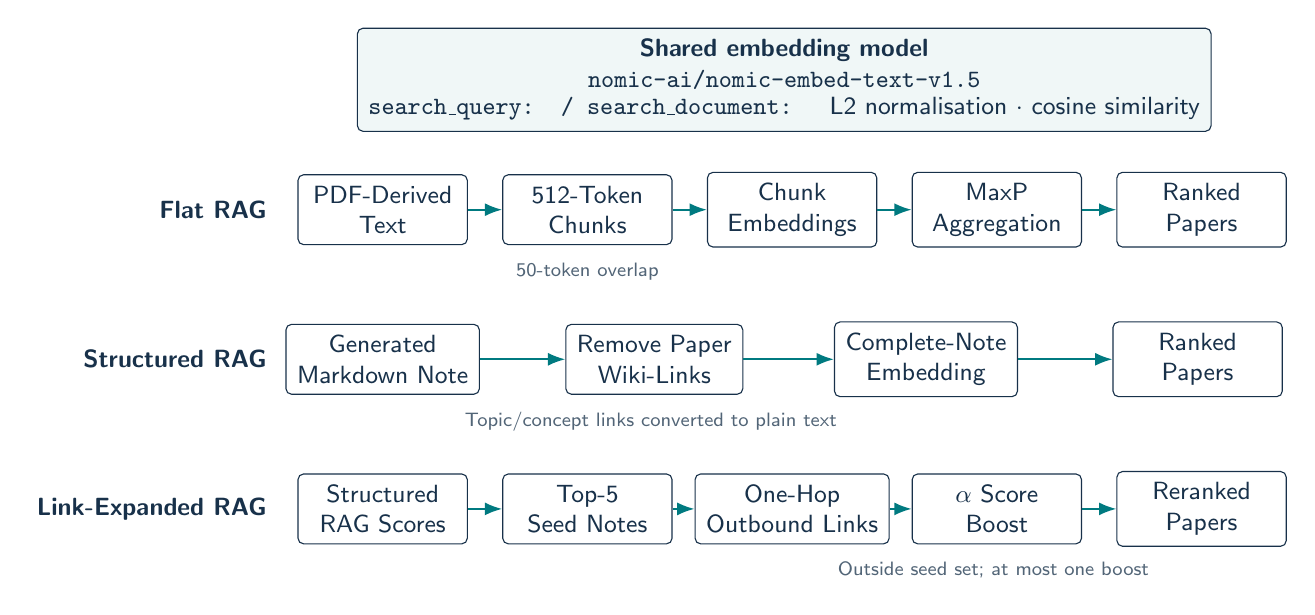
\begin{tikzpicture}[
        font=\sffamily\small,
        box/.style={
            draw=RetrievalNavy,
            text=RetrievalNavy,
            fill=white,
            rounded corners=2pt,
            align=center,
            minimum width=2.15cm,
            minimum height=0.82cm,
            inner sep=4pt
        },
        shared/.style={
            box,
            minimum width=9.7cm,
            fill=RetrievalTeal!6
        },
        rowlabel/.style={
            font=\sffamily\bfseries\small,
            text=RetrievalNavy,
            anchor=east
        },
        arrow/.style={
            -{Latex[length=2.2mm]},
            draw=RetrievalTeal,
            line width=0.7pt
        },
        note/.style={
            font=\sffamily\scriptsize,
            text=RetrievalNavy!75,
            align=center
        }
    ]

    % Shared model configuration
    \node[shared] (shared) at (7.3,0) {
        \textbf{Shared embedding model}\\
        \texttt{nomic-ai/nomic-embed-text-v1.5}\\[-1pt]
        \texttt{search\_query: / search\_document:}
        \quad L2 normalisation \(\cdot\) cosine similarity
    };

    % Flat RAG
    \node[rowlabel] at (0.85,-1.65) {Flat RAG};
    \node[box] (f1) at (2.2,-1.65) {PDF-Derived\\Text};
    \node[box] (f2) at (4.8,-1.65) {512-Token\\Chunks};
    \node[box] (f3) at (7.4,-1.65) {Chunk\\Embeddings};
    \node[box] (f4) at (10.0,-1.65) {MaxP\\Aggregation};
    \node[box] (f5) at (12.6,-1.65) {Ranked\\Papers};

    \draw[arrow] (f1.east) -- (f2.west);
    \draw[arrow] (f2.east) -- (f3.west);
    \draw[arrow] (f3.east) -- (f4.west);
    \draw[arrow] (f4.east) -- (f5.west);

    \node[note, below=1mm of f2] {50-token overlap};

    % Structured RAG
    \node[rowlabel] at (0.85,-3.55) {Structured RAG};
    \node[box] (s1) at (2.2,-3.55) {Generated\\Markdown Note};
    \node[box] (s2) at (5.65,-3.55) {Remove Paper\\Wiki-Links};
    \node[box] (s3) at (9.1,-3.55) {Complete-Note\\Embedding};
    \node[box] (s4) at (12.55,-3.55) {Ranked\\Papers};

    \draw[arrow] (s1.east) -- (s2.west);
    \draw[arrow] (s2.east) -- (s3.west);
    \draw[arrow] (s3.east) -- (s4.west);

    \node[note, below=1mm of s2] {
        Topic/concept links converted to plain text
    };

    % Link-Expanded RAG
    \node[rowlabel] at (0.85,-5.45) {Link-Expanded RAG};
    \node[box] (l1) at (2.2,-5.45) {Structured\\RAG Scores};
    \node[box] (l2) at (4.8,-5.45) {Top-5\\Seed Notes};
    \node[box] (l3) at (7.4,-5.45) {One-Hop\\Outbound Links};
    \node[box] (l4) at (10.0,-5.45) {\(\alpha\) Score\\Boost};
    \node[box] (l5) at (12.6,-5.45) {Reranked\\Papers};

    \draw[arrow] (l1.east) -- (l2.west);
    \draw[arrow] (l2.east) -- (l3.west);
    \draw[arrow] (l3.east) -- (l4.west);
    \draw[arrow] (l4.east) -- (l5.west);

    \node[note, below=1mm of l4] {
        Outside seed set; at most one boost
    };

    \end{tikzpicture}%
    }
    \caption{Retrieval configurations evaluated in RQ1. Flat RAG ranks
    papers through chunk-level retrieval and MaxP aggregation.
    Structured RAG embeds each generated note as one paper-level
    retrieval unit. Link-Expanded RAG reuses the Structured RAG scores
    and applies a one-hop score boost to eligible linked papers.}
    \label{fig:retrieval_configurations}
\end{figure}
}%

\subsubsection{Flat RAG}

The Flat baseline tokenises PDF-derived text using the embedding
model's tokenizer into sequential 512-token chunks with a 50-token
overlap. Each chunk \(c_j\) belonging to paper \(d_i\) is embedded
independently. No alternative chunk sizes or overlap values were
evaluated; these settings therefore define the fixed baseline
configuration. Paper-level scoring uses MaxP passage
aggregation~\cite{dai2019deeper}:

\[
\operatorname{Score}_{\mathrm{Flat}}(d_i,q)
=
\max_{c_j \in d_i}
\operatorname{sim}(q,c_j).
\]

Papers are ranked in descending order of this maximum score. A paper can
therefore rank highly when one passage strongly matches the query,
without requiring the complete paper to be represented by a single
embedding.

\subsubsection{Structured RAG}

Each complete agent-generated Markdown note \(n_i\) is treated as one
paper-level retrieval unit:

\[
\operatorname{Score}_{\mathrm{Struct}}(d_i,q)
=
\operatorname{sim}(q,n_i).
\]

Retrieval over summarised or higher-level representations has been
proposed as a means of preserving context that may be fragmented by
short, fixed-size passages~\cite{sarthi2024raptor}. The implementation
in this thesis is simpler than RAPTOR's hierarchical retrieval
architecture: one structured Markdown note represents each complete
paper.

Before embedding, paper-to-paper wiki-links are removed from the note
text. Wiki-links referring to general topics or concepts are converted
to plain text rather than removed. This preserves their textual meaning
while preventing the graph structure itself from contributing to the
Structured RAG similarity score.

The comparison between Flat RAG and Structured RAG therefore evaluates
a combined change from passage-level PDF-derived text to a paper-level,
LLM-generated representation. Since both retrieval granularity and
textual content change, the comparison should not be interpreted as
isolating a single causal effect of summarisation alone.

\subsubsection{Link-Expanded RAG}

This configuration begins with the same paper-level similarity scores
as Structured RAG. It then uses the outbound paper-to-paper wiki-links
generated by the Semantic Link Agent to apply a one-hop score boost.
This design is motivated by graph-assisted retrieval methods that
supplement vector similarity with explicit relationships between
information units~\cite{edge2024local}. However, the scoring rule
defined below is specific to the implemented pipeline and is not
presented as a standard GraphRAG scoring formula.

For each query \(q\), the five highest-ranked Structured RAG notes form
the seed set \(S_q\). The system follows the outbound paper-to-paper
wiki-links stored in those seed notes and identifies linked papers that
are present in the local corpus. Papers already in the seed set are not
eligible for a link boost.

Let \(N^{+}(S_q)\) denote the union of the one-hop outbound paper
neighbours of the seed notes. The set of eligible linked papers is:

\[
\widetilde{N}^{+}(S_q)
=
N^{+}(S_q)\setminus S_q.
\]

For cross-validation fold \(f\), the expanded score is:

\[
\operatorname{Score}_{\mathrm{Expanded}}^{(f)}(d_i,q)
=
\operatorname{Score}_{\mathrm{Struct}}(d_i,q)
+
\alpha_f
\mathbb{I}
\left(
d_i \in \widetilde{N}^{+}(S_q)
\right),
\]

where \(\mathbb{I}(\cdot)\) is the indicator function and
\(\alpha_f\) is the link-boosting coefficient selected for fold \(f\).

Because the graph contribution is represented by a binary indicator, a
paper receives the boost at most once even when it is linked from
multiple seed notes. Link traversal is restricted to one outbound hop
and is not applied recursively. Papers already present in the seed set
retain their original Structured RAG scores.

The coefficient was selected separately within five-fold stratified
cross-validation using shuffled splits and random seed \(42\), with
query categories used for stratification
~\cite{kohavi1995study}.

Candidate coefficients comprised \(0\) and, for each training query,
the positive score gaps between each top-five seed paper and each
eligible lower-scoring linked paper, plus \(10^{-8}\), rounded to eight
decimal places. Candidates were evaluated only on the training queries.
Selection prioritised MRR@5, followed by Recall@5, Precision@5, and the
smallest coefficient in the event of a tie.

The selected coefficient \(\alpha_f\) was applied unchanged to the
held-out queries in fold \(f\). Aggregating the five held-out rankings
produced one out-of-fold ranking for every query; a query's relevance
labels were therefore never used to select its own coefficient.

\FloatBarrier

\subsection{RQ1: Retrieval Evaluation}
\label{sec:rq1_method}

RQ1 compares Flat RAG, Structured RAG, and Link-Expanded RAG using 40 queries
manually constructed by the thesis author, who also identified the
papers considered relevant to each query using a binary relevance
criterion. The set contains 24 simple factual, eight comparison, and
eight neuro-symbolic queries. A paper was labelled relevant when a
reader familiar with the topic would expect it to help answer the query
and it contained substantive information directly addressing the query.
Each query had between one and six relevant papers.

Automated checks verified unique query identifiers, alignment between
the query and relevance files, and corpus membership of every labelled
paper. Query categories were used to stratify the five folds, and
evaluation was performed at paper level.



Let \(Q\) denote the set of evaluation queries, \(G_q\) the set of
papers judged relevant to query \(q\), and \(T_q^5\) the set of the five
highest-ranked papers. Query-level precision and recall at rank five are
defined as:

\[
P_5(q)
=
\frac{
    \left|T_q^5 \cap G_q\right|
}{5},
\]

\[
R_5(q)
=
\frac{
    \left|T_q^5 \cap G_q\right|
}{
    \left|G_q\right|
}.
\]

Let \(r_q\) denote the rank of the first relevant paper for query \(q\).
The truncated reciprocal-rank value is:

\[
RR_5(q)
=
\begin{cases}
\dfrac{1}{r_q},
& \text{if } r_q \leq 5,\\[0.8em]
0,
& \text{if no relevant paper occurs in the top five.}
\end{cases}
\]

The reported metrics are macro-averaged across all 40 queries:

\[
\operatorname{Precision@5}
=
\frac{1}{|Q|}
\sum_{q\in Q}P_5(q),
\]

\[
\operatorname{Recall@5}
=
\frac{1}{|Q|}
\sum_{q\in Q}R_5(q),
\]

\[
\operatorname{MRR@5}
=
\frac{1}{|Q|}
\sum_{q\in Q}RR_5(q).
\]

Macro-averaging gives every query equal weight regardless of the number
of relevant papers associated with it. Precision@5 measures the
relevance density of the returned ranking, Recall@5 measures how much
of the relevant set is recovered, and MRR@5 emphasises the position of
the first relevant paper.

Flat RAG and Structured RAG are evaluated directly over all 40 queries.
For Link-Expanded RAG, the reported metrics are calculated from the
aggregated held-out predictions of the five cross-validation folds.
Thus, the coefficient applied to each query is selected without using
that query's relevance labels.

The evaluation reports descriptive differences between the
configurations. No claims of statistical significance are made because
the study uses a focused set of 40 queries and does not include a
separate inferential significance-testing procedure.

\subsection{RQ2: Metadata and Topic Evaluation}
\label{sec:rq2_method}

RQ2 evaluates bibliographic metadata and semantic topic labels through
separate protocols.

\noindent\textbf{Bibliographic metadata.}
The bibliographic evaluation covers all 40 generated notes.
Agent-extracted metadata are compared with externally curated Semantic
Scholar records. Before comparison, wiki-links are reduced to their
canonical targets, strings are lowercased, punctuation is removed, and
whitespace is collapsed.

Titles and publication years are evaluated using normalised exact
matching. Author lists are treated as sets of normalised names and are
evaluated using precision, recall, and F1-score. Venue matching first
applies direct normalised matching, a fixed dictionary of known venue
synonyms, and acronym matching. When these checks fail, token-level
Jaccard similarity is calculated after removing years, digits, and
common connector words. A venue is accepted when this similarity is at
least \(0.70\). The bibliographic scores are macro-averaged across the
40 papers.

\noindent\textbf{Semantic topic labels.}
The semantic evaluation covers the 22 papers that overlap with the
supervisor's existing vault. Six paper titles stored among the expert
topic annotations are removed because they represent bibliographic
cross-references rather than semantic topic labels.

Two complementary protocols are used. First, a conservative strict
protocol compares the normalised agent-generated \texttt{hasTopic}
labels directly with the expert-authored labels for all 22 papers.
Precision, recall, and F1-score are calculated per paper and
macro-averaged.

Because strict lexical matching penalises synonymous expressions and
differences in topic granularity, a secondary canonicalised sensitivity
analysis examines how agreement changes when generated labels are mapped
to the expert vocabulary. After removing the six paper-title labels, the
set of expert label strings across all 22 papers forms a fixed vocabulary
of 49 canonical topics. This defines a closed-vocabulary mapping task
rather than an evaluation of generalisation to unseen topic labels. The
canonical and agent-generated labels are embedded using
\texttt{nomic-ai/nomic-embed-text-v1.5} with the
\texttt{clustering:} prefix and L2 normalisation.

Before mapping any agent-generated labels or calculating evaluation
scores, the mapping threshold is fixed using only the geometry of the
canonical vocabulary. Cosine similarities are calculated for all
\(\binom{49}{2}=1176\) distinct pairs of canonical labels. The
90th percentile of this distribution is used as the mapping threshold:

\[
\tau_m =0.7361
\]

This is an implementation-specific, vocabulary-relative heuristic
rather than a universal semantic-similarity threshold. It provides a
conservative cutoff anchored in the upper tail of the similarity
distribution within the expert vocabulary. An agent label is assigned
to its nearest canonical label only when their cosine similarity is at
least \(\tau_m\); otherwise, it is discarded.

The 22 papers are divided deterministically into seven development
papers and a 15-paper evaluation subset. The split is stratified by the
number of expert topic labels attached to each paper. Within each
stratum, papers are ordered by arXiv identifier, with approximately one
third assigned to development and the remainder to evaluation.

The vocabulary and \(\tau_m\) are defined globally using annotations
across all 22 papers. The 15-paper evaluation subset is held out only
from selection of \(\tau_d\) and \(k\).

Two further parameters are selected using only the development set.
After topic mapping, \(\tau_d\) controls the removal of semantically
near-duplicate canonical labels, while \(k\) limits the maximum number
of canonical topics retained for each paper. The near-duplicate
threshold is evaluated over

\[
\tau_d \in \{0.85,0.90,0.95\},
\]

and the maximum number of retained canonical topics is evaluated over

\[
k \in \{3,4,5\}.
\]

For each combination, canonicalised exact-match F1 is calculated per
development paper and macro-averaged. The combination with the highest
development macro-F1 is selected, resulting in
\(\tau_d=0.85\) and \(k=4\). These values are then frozen and applied
unchanged to the 15-paper evaluation subset. Holding this subset out
from selection of \(\tau_d\) and \(k\) reduces the risk of selection
bias caused by optimising these parameters on the final evaluation
observations~\cite{cawley2010overfitting}.

The canonicalised protocol is reported as a secondary closed-vocabulary
sensitivity analysis on the 15-paper evaluation subset; it does not
replace the strict lexical protocol. Because the two protocols use
different matching procedures and sample sizes, their scores are
reported separately and are not interpreted as directly comparable
estimates. OpenAlex topics and keywords are used only as supplementary
evidence and do not affect either reported score.

\subsection{RQ3: Citation Reference Evaluation}
\label{sec:rq3_method}

RQ3 evaluates a batched citation-extraction pipeline that attempts to
process each detected reference section in full and applies
deterministic per-entry fallback parsing when LLM batch outputs are
unavailable. It processes explicit bibliography entries and remains
separate from the Semantic Link Agent, which infers conceptual
relationships between local papers.

For each paper, the pipeline reads the PDF-derived text from its JSON
record and searches for a reference-section heading. In the evaluated
corpus, a heading was detected for all 40 papers. The complete remaining
text from that heading was segmented using bracketed numeric markers and
numbered reference entries; continuation lines were joined until the
next reference marker. The resulting entries were divided into batches
of at most 30.

The agent is instructed to return structured records containing, where
available, a title, authors, publication year, venue, DOI, arXiv
identifier, and Semantic Scholar identifier. Empty responses, failed
batches, and batches skipped after activation of the quota or
rate-limit circuit breaker are processed through a deterministic
fallback parser. The parser attempts to recover a title-like string
from each raw bibliography entry while leaving unavailable fields
empty.

The fallback parser is not applied to every malformed structured
record. Before scoring, records lacking every usable identifier and a
usable normalised title are removed according to predefined validation
rules. The remaining records are deduplicated using Semantic Scholar
identifiers, DOIs, arXiv identifiers, and normalised titles.

When an extracted reference matches one of the 40 corpus papers, a
subsequent local-resolution step can additionally attach an Obsidian
wiki-link. References outside the local corpus remain valid extraction
outputs.

The outgoing reference lists returned by the Semantic Scholar Academic
Graph are used as the offline gold standard
~\cite{kinney2023semantic}. Semantic Scholar is not queried by the
Citation Link Agent during extraction. External citations are retained,
so the evaluation is not restricted to references pointing to papers
within the local corpus.

Predicted and gold references are matched one-to-one in the following
priority order:

\begin{enumerate}
    \item Semantic Scholar identifier;
    \item DOI;
    \item arXiv identifier; and
    \item normalised exact title.
\end{enumerate}

Once a gold record is matched, it cannot be matched again. Approximate
title matches are retained only for audit purposes and do not contribute
to the scores.

Precision, recall, and F1-score are calculated from pooled
true-positive, false-positive, and false-negative counts across the
scored papers. Three papers without usable Semantic Scholar gold
reference lists are excluded, leaving 37 papers in the final
evaluation. No paper is excluded because of a provider block. Empty
predictions that remain within the scored set are treated as extraction
failures and therefore contribute false negatives.

Full-section input processing, bibliography segmentation, batching,
availability handling, and deterministic per-entry fallback parsing
operate jointly. The reported result therefore characterises the
extraction pipeline as a whole rather than an isolated test of input
truncation.

\subsection{RQ4: Expert Evaluation}
\label{sec:rq4_method}

RQ4 uses a completed exploratory expert evaluation of five papers
selected by simple random sampling without replacement from the sorted
corpus identifiers using a fixed random seed of \(42\). The selected
document identifiers are retained with the evaluation artefacts. For each paper, the supervisor received the paper
title and abstract, access to the complete PDF, and the full
agent-generated Markdown note.

Each note was rated on a five-point Likert scale
(\(1=\) unacceptable; \(5=\) excellent) across four dimensions:

\begin{enumerate}
    \item factual faithfulness;
    \item core-contribution coverage;
    \item structure and readability; and
    \item utility for rediscovery.
\end{enumerate}

The individual paper-level ratings, arithmetic mean for each dimension,
overall mean across all ratings, and optional qualitative comments are
reported descriptively. The dimensions are informed by established
human-evaluation practices for generated summaries
~\cite{fabbri2021summeval}.

Because the evaluation contains one expert and five generated notes, no
inferential statistical analysis is performed. The findings are treated
as an exploratory expert assessment of the current pipeline rather than
as a generalisable user study.

\subsection{Reproducibility and Experimental Controls}
\label{sec:reproducibility}

Corpus-alignment assertions verified consistent identifiers across
extracted texts, generated notes, retrieval queries, expert annotations,
and evaluation outputs. Embeddings, external gold records, and LLM
predictions were cached to avoid unnecessary recomputation and variation
from repeated provider calls.

For RQ1, the queries, relevance labels, cross-validation folds, selected
coefficients, and held-out predictions were retained. For RQ2, the
canonical vocabulary, pairwise-similarity summary, mapping threshold,
development and evaluation-subset identifiers, development grid, selected parameters,
and mapping decisions were retained. For RQ4, the sampling procedure,
selected identifiers, rating dimensions, expert responses, paper-level
scores, and qualitative comments were retained.

RQ3 provenance records the configured Gemini Flash-family model pool,
temperature \(0.0\), prompt version \texttt{v1}, generation timestamp,
and a SHA-256 hash of the shared citation-extraction source module. The
final experimental driver containing the batching and fallback
procedures was also retained. The first requested alias was
\texttt{gemini-flash-latest}; the wrapper could rotate among configured
Flash-family endpoints following quota or rate-limit errors. Because the
resolved endpoint was not logged for each request, exact hosted-model
replication remains limited.

Version-controlled prompts, input-processing rules, source code, and
experimental drivers were retained in the project repository.
Evaluation artefacts were retained separately. For RQ3, raw responses
were stored alongside structured predictions, per-paper records, and
aggregate results. Predefined rules handled empty or invalid outputs,
unavailable gold data, and provider failures rather than manual score
adjustment.

Generated notes, semantic links, and RQ1 and RQ2 artefacts remained
frozen throughout the final RQ3 evaluation; RQ3 therefore could not
alter the earlier artefacts or results.

\FloatBarrier

% ============================================================
\section{Results}
\label{sec:results}
% Placeholder for Section 4: Results
% Guideline: Present the main results of analysis/implementation, explaining how they 
% address the problem. Situate results in the context of reviewed literature, supporting 
% conclusions with clear arguments and evidence.

This section presents the results for retrieval performance (RQ1),
metadata and topic extraction accuracy (RQ2), citation-reference
extraction accuracy (RQ3), and the exploratory expert evaluation of
generated-note quality (RQ4).

\subsection{RQ1: Retrieval Performance}
\label{sec:rq1_results}

Flat RAG and Structured RAG were evaluated across all 40 queries.
Link-Expanded RAG reports the aggregated held-out predictions obtained
through five-fold cross-validation. Table~\ref{tab:rq1_results}
presents the macro-averaged retrieval metrics.

\begin{table}[!htbp]
\centering
\caption{Retrieval performance across the three configurations.}
\label{tab:rq1_results}
\begin{tabular}{lccc}
\toprule
\textbf{Configuration} & \textbf{Recall@5} & \textbf{Precision@5} & \textbf{MRR@5} \\
\midrule
Flat RAG & 0.696 & \textbf{0.235} & 0.729 \\
Structured RAG & 0.696 & 0.225 & \textbf{0.744} \\
Link-Expanded RAG & \textbf{0.719} & 0.230 & 0.742 \\
\bottomrule
\end{tabular}
\end{table}

Structured RAG achieved the same Recall@5 as Flat RAG. Its Precision@5
decreased from 0.235 to 0.225, while MRR@5 increased from 0.729 to
0.744. Thus, the structured-note representation did not improve
retrieval coverage, but the first relevant paper tended to occur higher
in the ranking.

Link-Expanded RAG produced the highest observed Recall@5 at 0.719,
compared with 0.696 for both Flat RAG and Structured RAG. Its
Precision@5 was 0.230, and its MRR@5 was 0.742. Both values lay between
the corresponding Flat RAG and Structured RAG results.

\subsection{RQ2: Metadata and Topic Evaluation}
\label{sec:rq2_results}

RQ2 comprises a bibliographic metadata evaluation over all 40 papers
and two semantic-topic evaluation protocols over the 22 papers that
overlapped with the expert-authored topic annotations.

\subsubsection{Bibliographic Metadata}

Table~\ref{tab:rq2_group_a} reports the comparison between the
agent-extracted bibliographic fields and the Semantic Scholar records.

\begin{table}[!htbp]
\centering
\caption{Bibliographic metadata extraction results over 40 papers.}
\label{tab:rq2_group_a}
\begin{tabular}{lc}
\toprule
\textbf{Metadata field} & \textbf{Score} \\
\midrule
Title exact match & 0.975 \\
Year exact match & 0.775 \\
Venue fuzzy match & 0.500 \\
Author-set F1 & 0.825 \\
\bottomrule
\end{tabular}
\end{table}

The highest result was obtained for title extraction, with an exact
match rate of 0.975. Author extraction achieved an F1-score of 0.825,
based on a precision of 0.822 and recall of 0.829. The year exact-match
rate was 0.775, while venue matching produced the lowest bibliographic
score at 0.500.

\subsubsection{Semantic Topic Labels}

After removing six full paper-title labels that represented
bibliographic cross-references rather than concept labels, strict
normalised set matching was applied over the 22 overlapping papers.

A secondary closed-vocabulary canonicalised sensitivity analysis used
seven development papers and a separate 15-paper evaluation subset.
The fixed 49-label expert vocabulary was derived from annotations
across all 22 papers, and \(\tau_m=0.7361\) was calculated from
similarities within that vocabulary. Only \(\tau_d=0.85\) and \(k=4\)
were selected on the development subset and then applied unchanged to
the 15-paper evaluation subset.

\begin{table}[!htbp]
\centering
\caption{Semantic topic-label evaluation results.}
\label{tab:rq2_topic_results}
\begin{tabular}{lcccc}
\toprule
\textbf{Protocol} & \textbf{Papers} & \textbf{Precision} & \textbf{Recall} & \textbf{F1} \\
\midrule
Strict topic overlap & 22 & 0.076 & 0.151 & 0.096 \\
Canonicalised 15-paper subset & 15 & 0.339 & 0.476 & 0.383 \\
\bottomrule
\end{tabular}
\end{table}

The strict and canonicalised scores are not directly comparable because
the protocols use different matching procedures and evaluation subsets;
the canonicalised result is reported as a secondary sensitivity
analysis.

\subsection{RQ3: Citation Reference Evaluation}
\label{sec:rq3_results}

The citation-extraction pipeline was evaluated against outgoing
reference lists obtained from Semantic Scholar. Of the 40 corpus papers, three did not
have usable gold reference data. No papers were excluded because of a
provider-block status. The final evaluation therefore scored 37 papers.
Two in-scope papers produced no usable predictions because their model
responses were truncated. They remained in the scored set, increasing
the pooled false-negative count.

\begin{table}[!htbp]
\centering
\caption{Citation-reference extraction performance over 37 scored papers.}
\label{tab:rq3_results}
\begin{tabular}{lcccccc}
\toprule
\textbf{Task} & \textbf{TP} & \textbf{FP} & \textbf{FN} & \textbf{Precision} & \textbf{Recall} & \textbf{F1} \\
\midrule
Citation extraction & 1,514 & 283 & 534 & 0.843 & 0.739 & 0.788 \\
\bottomrule
\end{tabular}
\end{table}

The pipeline achieved higher precision than recall. This
indicates that most extracted references matched the Semantic Scholar
gold records, while some gold references were still missed.

Among the 1,514 true-positive matches, 107 were resolved through DOI
identifiers, 463 through arXiv identifiers, and 944 through normalised
exact-title matches. No matches were established directly through a
Semantic Scholar paper identifier. In total, 57 invalid agent output
records were filtered before scoring.

\subsection{RQ4: Exploratory Expert Evaluation}
\label{sec:rq4_results}

RQ4 used an exploratory expert evaluation of five generated notes. The
same expert rated each note on factual faithfulness, core-contribution
coverage, structure and readability, and utility for rediscovery using a
five-point Likert scale. Table~\ref{tab:rq4_results} reports the
paper-level ratings and dimension means.

\begin{table}[!htbp]
\centering
\caption{Expert ratings for generated-note quality.}
\label{tab:rq4_results}
\begin{tabular}{lcccc}
\toprule
\textbf{Paper ID} & \textbf{Faithfulness} & \textbf{Coverage} & \textbf{Readability} & \textbf{Utility} \\
\midrule
2305.19951 & 4 & 3 & 4 & 4 \\
2005.11401 & 4 & 3 & 4 & 3 \\
2402.12240 & 4 & 3 & 3 & 3 \\
2401.15884 & 3 & 2 & 3 & 2 \\
2401.05224 & 4 & 4 & 3 & 4 \\
\midrule
Mean & 3.8 & 3.0 & 3.4 & 3.2 \\
\bottomrule
\end{tabular}
\end{table}

The overall mean across the 20 ratings was 3.35. The strongest dimension
was factual faithfulness, while core-contribution coverage received the
lowest mean score. The qualitative comments repeatedly noted excessive
wiki-linking and incomplete explanations of methodology or limitations.
Because the evaluation used one expert and five notes, these results are
reported as exploratory evidence rather than as a generalisable user
study.

% ============================================================
\section{Discussion}
\label{sec:discussion}

This section interprets the experimental findings, relates them to the
research questions, and discusses the main methodological limitations of
the study.

\subsection{Structured and Link-Expanded Retrieval}

The observed differences between Flat and Structured RAG were modest. Structured RAG achieved the
same Recall@5 as Flat RAG (0.696), slightly lower Precision@5 (0.225
compared with 0.235), and higher MRR@5 (0.744 compared with 0.729).
This partly supports the motivation for representing papers as
structured notes: the first relevant paper tended to occur higher in the
ranking, but retrieval coverage did not improve. One possible
explanation is that a generated note concentrates paper-level
information into a more compact representation than raw PDF chunks.
However, the experiment did not directly measure information density,
chunk noise, or which note sections contributed most to retrieval
performance~\cite{lewis2020retrieval,sarthi2024raptor}.

Link-Expanded RAG produced the highest observed Recall@5 (0.719),
compared with 0.696 for both Flat RAG and Structured RAG. Its
Precision@5 and MRR@5 lay between the corresponding Flat RAG and
Structured RAG results. The higher observed Recall@5 is consistent with one-hop wiki-link
expansion retrieving some additional relevant papers in this corpus,
but the difference was small and was not accompanied by improvements
across all metrics. Compared with heavier graph-based
RAG systems, the approach used here is deliberately lightweight: it
operates over local Markdown links rather than a separately extracted
entity graph or external graph database~\cite{edge2024local,gutierrez2024hipporag}.
Without confidence intervals or significance tests, these differences
should be interpreted descriptively rather than as evidence that one
configuration is generally superior~\cite{urbano2019statistical}.

\subsection{Metadata and Topic Extraction}

The RQ2 results show different levels of performance for bibliographic
metadata extraction and semantic topic alignment. Bibliographic fields were comparatively reliable: title exact matching reached 0.975 and
author-set F1 reached 0.825. Year extraction was lower at 0.775, and
venue matching was the weakest bibliographic field at 0.500. This may reflect differences between preprint metadata visible in PDFs and the
version-of-record metadata stored by Semantic Scholar, as well as
variation in venue abbreviations and naming conventions.

Topic alignment was substantially harder. Strict topic matching over
the 22 papers overlapping with the expert-authored vault produced an
F1-score of 0.096. The separate closed-vocabulary canonicalised
sensitivity analysis yielded an F1-score of 0.383 on its 15-paper
evaluation subset after mapping agent labels into the fixed expert
vocabulary. The higher score is consistent with vocabulary and schema
mismatch contributing to low strict overlap, but it does not quantify
that contribution because the protocols and subsets differ. The
canonicalised result therefore complements rather than replaces the
strict result~\cite{furnas1987vocabulary,balog2019personal}.

\subsection{Citation Reference Extraction}

The final RQ3 evaluation yielded a precision of 0.843, recall of 0.739,
and F1-score of 0.788 across 37 scored papers. The evaluation included two papers whose truncated model responses
yielded no usable predictions; their missed references contributed to
the pooled false-negative count.

The match-type breakdown shows that normalised exact-title matching was
central to the evaluation: 944 of the 1,514 true positives were matched
through exact titles, compared with 107 through DOI identifiers and 463
through arXiv identifiers. Title normalisation was therefore important
under the matching procedure; an identifier-only procedure would have
credited substantially fewer matches. At the same time, dependence on
title matching makes the system sensitive to title variants and
extraction noise. This situates the task within literature spanning
conventional scientific-document extraction pipelines such as
CERMINE~\cite{tkaczyk2015cermine} and LLM-based schema-guided
information extraction~\cite{xu2024large}.

\subsection{Expert Evaluation of Generated Notes}

The RQ4 expert evaluation provides exploratory evidence about the
quality of the generated notes. The strongest dimension was factual
faithfulness, with a mean score of 3.8 out of 5. Structure and
readability reached 3.4, utility for rediscovery reached 3.2, and
core-contribution coverage was lowest at 3.0. The qualitative comments
identified repeated issues with excessive wiki-linking, unclear
methodological explanations, and weak limitation sections.

The notes were generally rated as factually faithful, but only
moderately useful for rediscovery and inconsistent in capturing the
methodological substance expected by the expert. This is important
because the pipeline is intended for academic rediscovery rather than
only for generic summarisation. A note can receive a favourable
faithfulness rating while still being insufficiently useful for an
expert research workflow. Because RQ4 used one expert and five notes,
the findings should be treated as exploratory rather than as a
generalisable user study~\cite{fabbri2021summeval}.

\subsection{Limitations}

Several limitations bound the findings of this study:

\begin{itemize}
    \item \textbf{Corpus and Query Scope:}
    The study uses one 40-paper personal research collection and
    40 queries. Although this controlled corpus enables direct comparison
    between retrieval configurations, it limits the external validity of
    the findings.

    \item \textbf{Annotation Reliability:}
    RQ1 relevance judgements, RQ2 expert topic labels, and RQ4 note
    ratings were each based on a single annotator or expert source. No
    independent duplicate annotation was available, so inter-annotator
    agreement could not be assessed.

    \item \textbf{Descriptive Retrieval Comparisons:}
    RQ1 reports macro-averaged scores without confidence intervals or
    significance tests, so differences are descriptive within the
    evaluated query set. The comparison also uses one embedding model,
    chunking configuration, and link-expansion rule. Individual semantic
    links were not assessed against an edge-level gold standard; only
    the aggregate downstream retrieval effect of the link-expansion
    configuration was measured.

    \item \textbf{Construct Validity of Topic Matching:}
    Strict normalised label overlap primarily measures vocabulary
    agreement rather than complete conceptual alignment. The
    canonicalised sensitivity analysis instead assumes a closed
    vocabulary derived from all 22 annotated papers and heuristic
    mapping and deduplication thresholds.

    \item \textbf{RQ3 Evaluation Coverage:}
    The citation-reference evaluation depends on Semantic Scholar coverage
    and record quality and is limited to the 37 scored papers with usable
    gold reference lists. Two in-scope papers produced no usable predictions
    because their model responses were truncated and were retained as
    extraction failures.

    \item \textbf{RQ4 Evaluation Scope:}
    The evaluation contains five generated notes assessed by one expert.
    It should therefore be treated as an exploratory expert assessment
    rather than a generalisable user study.

    \item \textbf{Hosted LLM Reproducibility:}
    The LLM-backed stages used a hosted Gemini Flash-family model pool
    with temperature fixed at \(0.0\). Because the resolved model
    endpoint was not logged for each request, exact reproduction of
    model behaviour is limited.
\end{itemize}

\subsection{Future Work}

Future work should test larger and more diverse collections and quantify
RQ1 uncertainty using bootstrap confidence intervals or paired
query-level significance tests~\cite{urbano2019statistical}. Multiple
annotators should evaluate relevance judgements, topic labels, and
generated notes.

The difference between the strict and canonicalised topic results
motivates incorporating a researcher's vocabulary during topic
generation or downstream alignment, while reporting strict and mapped
results separately. The lower RQ4 coverage score and qualitative
comments motivate prompts that emphasise methodology and limitations
and stricter wiki-link filtering. Ablations should separate note
structure from retrieval granularity and compare alternative chunking
and link-expansion rules.

Finally, the hosted pipeline should be compared with a fixed-version
local open-weight model to improve control over model versions, reduce
provider dependence, and keep document processing local.

% ============================================================
\section{Conclusion}
\label{sec:conclusion}

\paragraph{Main objective.}
This thesis evaluated a modular LLM-based pipeline that transforms
academic PDFs into structured, interlinked Obsidian Markdown notes and
assessed its retrieval, extraction, and note-quality performance.

\paragraph{Summary of findings.}
Structured RAG did not consistently outperform Flat RAG: Recall@5 was
unchanged, Precision@5 decreased slightly, and MRR@5 increased.
Link-Expanded RAG achieved the highest Recall@5 at 0.719, providing
partial support for H1. Bibliographic fields showed stronger agreement
with reference records than generated topic labels showed with expert
annotations, supporting H2, although venue extraction and strict topic
matching remained weak. The citation-extraction pipeline achieved a precision of 0.843 and lower
recall of 0.739, consistent with H3; its F1-score was 0.788. The exploratory expert evaluation produced an overall mean of 3.35 out
of 5; factual faithfulness scored highest, while core-contribution
coverage equalled the neutral midpoint at 3.0. As H4 required all four
dimension means to exceed 3.0, it was not fully supported.

\paragraph{Contribution and conclusion.}
The main contribution is an implemented and empirically evaluated
academic-paper ingestion pipeline that compares flat chunk retrieval
with structured-note retrieval and evaluates one-hop semantic-link
expansion as an additional ranking step. Within the focused 40-paper
collection, the pipeline achieved its strongest results on title,
author, and citation-reference extraction. However, structured notes
alone yielded mixed retrieval results, while topic alignment and note
coverage remained incomplete.

% ============================================================
\section*{Addendum: Reflection}
\label{sec:reflection}

The main lesson from this project was that system optimisation and
scientific evaluation require different decisions. If this had been
purely a production project, I could have repeatedly changed prompts,
mappings, filters, and other components whenever a result appeared
weak. In the thesis, however, adapting the system after observing
evaluation outcomes would have made those results difficult to defend.
I therefore separated the components into explicit evaluation
protocols, preserved unfavourable results, and distinguished primary
evaluations from secondary sensitivity analyses.

Discussions with my supervisor, together with the repositories and
examples he shared, helped me refine the scope and distinguish more
clearly between system development and scientific evaluation.

This tension was clearest in the topic-alignment evaluation. Rather than
continuing to modify the pipeline after observing low strict overlap, I
retained the expert-label comparison as the primary result and used
canonicalisation only as a secondary sensitivity analysis. This
preserved the weaker result while showing that strict overlap was
sensitive to the vocabulary used in the expert vault; the two protocols
therefore answer related but different questions.

I also underestimated the time required to freeze experimental
artefacts, reconcile outputs across pipeline stages, and verify that
later changes had not altered earlier evaluations. Defining the
evaluation boundaries and artefact-retention rules earlier would have
reduced rework and made the final phase more efficient.

If I restarted the project, I would obtain topic annotations from more
than one annotator and include a fixed-version local open-weight model
as an additional condition to reduce dependence on hosted provider
behaviour.

\par\noindent\textbf{Code and artefacts: }
\href{https://github.com/vonargeus/llm-academic-pkm-pipeline}
{\texttt{GitHub repository}}

\bibliographystyle{splncs04}
\bibliography{refs}

\end{document}
